\documentclass{scrartcl}
\usepackage{graphicx}
\usepackage{float}
\usepackage{amsmath}
\usepackage{verbatim}
\usepackage{caption}
\usepackage{subcaption}
\usepackage{hyperref}
\usepackage{amsfonts}

\DeclareOldFontCommand{\rm}{\normalfont\rmfamily}{\mathrm}

\newcommand{\figwidth}{4in}
\newcommand\tab[1][0.5cm]{\hspace*{#1}}
\renewcommand\thesubsection{\thesection.\alph{subsection}}

\newcommand{\R}{\mathbb{R}}

\title{Research Skills for Computational Applied Mathematics}
\subtitle{Matlab documentation}

\begin{document}

\begin{titlepage}
\author{Dr. Zofia Trstanova\\zofia.trstanova@ed.ac.uk \and Dr. Kostas Zygalakis\\ k.zygalakis@ed.ac.uk}


\clearpage\maketitle
\thispagestyle{empty}
\end{titlepage}

\newpage
\setcounter{page}{1}

\section{Introduction}
This project strictly follows~\cite{sanz2014markov}. The programming exercises are written in Matlab code available at \url{https://github.com/ZofiaTr/MCMC_SanzSerna}.

The main source code is located in folder "Matlab$\_$code". The exercise tasks $1-6$ correspond to functions called "main$+$task$\_$number$+$task$\_$name ". Functions used in the main files are saved in folder "functions", which is linked by "addpath" command at the beginning of each file. Figures are saved in folder "figures".

For MATLAB documentation, see \url{https://uk.mathworks.com/help/matlab/} or type
\begin{verbatim}
help commandYouWantToKnowAbout
\end{verbatim}
in MATLAB. 

Other useful tools for writing the report and presentations are \LaTeX and beamer package, see \url{https://en.wikibooks.org/wiki/LaTeX/Presentations}. You can create a project on \url{overleaf.com},  there are many \LaTeX  templates available.

\section{Metropolis Random Walk}

\subsection{Histogram}
The source code is in "main1$\_$sample$\_$MetropolisRW.m". The simulation is described in~\cite{sanz2014markov}[Section 5.3 ] and it reproduces~\cite{sanz2014markov}[Figure 6].

The following code implements one dimensional Metropolis random walk, i.e. for $N$ simulation steps, the new state $X^{n+1}$ is obtained from the previous state $X^{n}$ using the proposal
\[
\tilde{X}^{n+1} = X^n + h Z^n,
\]
where $h>0$ is the step size, $Z_n$ are independent identically distributed continuous random variables in $\R^d$ with $d=1$ according to a normal (Gaussian) distribution $\mathcal{N}(0,1)$. The new state is then obtained by Metropolis rule, which defines the acceptance probability $a$ for $\tilde{X}^{n+1}$ as
\[
a  = {\rm min}\left(1, \frac{\rho(\tilde{X}^{n+1})}{\rho(X^n)}\right).
\]
If the proposal is accepted, we set $X^{n+1}=\tilde{X}^{n+1}$, otherwise if the proposal is refused, we set $X^{n+1}=X^{n}$. 

In the following example, we use this algorithm to sample from the Boltzmann distribution with density
\begin{equation}
\rho(x) = Z^{-1}{\rm e}^{-\beta x^4},
\label{quartic}
\end{equation}
where $\beta$ is the inverse temperature and $Z$ is the normalization constant such that
\[
\int_{\R} \rho(x)dx = 1.
\]

The code begins with a common practice in MATLAB to clear all the objects in the workspace, close all figures and clear the command window.
\begin{verbatim}
clear all;
close all;
clc;
\end{verbatim}
The simulation parameters and the distribution are defined in this section, see their description inside the MATLAB comments.
\begin{verbatim}
% number of steps 
N = 1000000;
% step size
h = 1.0;
%inverse  temperature 
beta = 1.0;

% potential
V = @(x) x.^4;
% target probability density
rho = @(x) exp(-beta .*V(x));
\end{verbatim}
It is possible to define the random number generator by fixing the seed. The code then produces the same sequence of random numbers at every execution. This can be useful for example for debugging.
\begin{verbatim}
seed=0;
rng(seed);
\end{verbatim}
Once we have initialized the arrays to store the samples, we can start the main iteration of $N$ steps to perform the sampling. Note that for small systems, it is more efficient to precompute the array of random numbers.
\begin{verbatim}
% initialize array of samples
X = zeros(1, N); 
% intialize randon numbers, see help randn, help rand
Z = randn(1, N);
U = rand(1, N);

fprintf('Sampling RW\n')

for n = 1 : N - 1    
    % proposal 
    X(n+1) = X(n) + h * Z(n);
    
    %Metropolis step: acceptance ratio
    acceptanceRatio = rho(X(n+1)) / rho(X(n));
    
    % metropolis rule
    if (acceptanceRatio < U(n+1))
        % refuse
        X(n+1) = X(n);
    end
    
end
fprintf('sampling done\n')
\end{verbatim}
Note that the Metropolis rule tests the condition that the proposal is rejected. Since we have already assigned the proposal to the array $X$ at index $n+1$ in the line before, if the proposal is accepted, there is nothing to be done. Testing the refusal condition is more efficient, because in the case of refusal we only assign the value from the previous step to $X_{n+1}$.

In the postprocessing part, we create a histogram of samples $X^n$. Note that in order to make all figures consistent, it is a good idea to define parameters, which, for example, fix the font size. 
\begin{verbatim}
%% show histogram
myFontSize = 14;

f6 = figure(6);
h = histogram(X, 20, 'Normalization','probability');
xlabel('X', 'FontSize', myFontSize)
ylabel('Probability', 'FontSize', myFontSize)
set(gca, 'FontSize', myFontSize)

%save the figure
print(f6,'figures/figure6','-dpng')
\end{verbatim}

\subsection{Tasks}
\begin{enumerate}
\item Plot the trajectory $X^n$ over $n $ steps.
\item Fit the target density into the histogram.
\item Comment out the Metropolis step, and rerun the sampling only with the random walk proposal, create plot of $X^n$ over $n $ steps. 
\end{enumerate}


\section{Autocorrelation}

The source code is in "main2$\_$sample$\_$autocorrelation.m". The simulation reproduces~\cite{sanz2014markov}[Figure 7].

This code performs the sampling of the distribution~\eqref{quartic} by Random Walk Metropolis Algorithm (see previous section). The main difference with the structure of \\ "main1$\_$sample$\_$MetropolisRW.m" is that the sampling part is wrapped up as a function called "sample$\_$MetropolisRW" which is saved in folder "functions". This function takes number of steps to be performed $N$, steps size $h$, distribution that should be sampled $\rho$ and initial state $X_0$ and returns an array of $N$ samples $X$ and an array of rejections of size $N$.
\begin{verbatim}
function [X, rejections] = sample_MetropolisRW(N, h, rho, X0)
% parameters :
%  
%   number of steps N
%   stepsize h
%   rho is target density
%   initial condition X_0, size(1, d)
% return : trajectory and number of rejections

% determine dimension from the initial condition
d = length(X0);
% initialize array of samples
X = zeros(d, N); 
X(:,1) = X0;
rejections = 0;

% intialize randon numbers, see help randn, help rand
Z = randn(d, N);
U = rand(1, N);

for n = 1 : N - 1   
    % proposal 
    X(:,n+1) = X(:,n) + h * Z(:,n);    
    %Metropolis step: acceptance ratio
    acceptanceRatio = rho(X(:,n+1)) / rho(X(:,n));    
    % random number    
    if (acceptanceRatio < U(n+1))
        % refuse
        X(:,n+1) = X(:,n);
        rejections = rejections+1;
    end
end
end
\end{verbatim}

The main code "main2$\_$sample$\_$autocorrelation.m" then calls this function to generate samples. The first part of the code is as before:
\begin{verbatim}
% clean the working space
clear all;
close all;
clc;

addpath([pwd,'/functions']);

% choose initial seed, comment out to turn off, see help rng
seed=0;
rng(seed);
myFontSize = 14;

%inverse  temperature 
beta = 1.0;
% potential
V = @(x) x.^4;
% target probability density
rho = @(x) exp(-beta .*V(x));
\end{verbatim}
We want to investigate several step sizes, we therefore have an array of step sizes $h$, which will be iterated over later on.
\begin{verbatim}
% step size
h = [0.5, 1, 2, 4];
% number of various stepsizes
nrh = length(h);
% number of steps 
N = 1000000;
%initial condition 
X0=0;
\end{verbatim}
In order to compute the empirical auto-covariance, we choose the lag array. We also initialize a figure to allow writing inside during the iterations over the step sizes.
\begin{verbatim}
lag  = 0:19;

f7 = figure(7);
hold on
% initialize for loop counter
i=0;
\end{verbatim}
What follows is the main for-loop over the step sizes: for every step size $h$, we perform the sampling and compute the empirical auto-correlation. The implementation of the function \textit{compute$\_$empirical$\_$auto$\_$correlation$\_$coeff} is one of the tasks (see the end of this section). Finally, within each iteration, we plot the auto-covariance in a subplot belonging to the pre-intialized figure.
\begin{verbatim}
for stepSize = h 
    fprintf('Sampling with step size h = %f\n', stepSize);
    % increase the loop counter
    i = i+1;
   % perform the sampling with given parameters	
    [X, rejections] = sample_MetropolisRW(N, stepSize, rho, X0);
    %%%%% compute_empirical_auto_correlation_coeff
    rho_nu = compute_empirical_auto_correlation_coeff(X, lag);
    %%%%%%%%%%%%%%%%%%%%%%%
    
    subplot(2,2,i)
    plot(lag, rho_nu, 'LineWidth', 2)
    xlabel('lag', 'FontSize', myFontSize)
    ylabel('Correlation', 'FontSize', myFontSize)
    ylim([0,1])
    xlim([0,max(lag)])
    legend(['h = ', num2str(stepSize)])
    title([num2str(rejections), ' rejections, rate ', num2str(rejections / length(X))])
    set(gca, 'FontSize', myFontSize)

end
%% save figure
print(f7,'figures/figure7','-dpng')
\end{verbatim}


\subsection{Tasks}
\begin{enumerate}
\item Implement auto-covariance function called "compute$\_$empirical$\_$auto$\_$correlation$\_$coeff" which takes array of samples $X$ and lag and returns empirical auto-covariance computed according to the formula at the end of~\cite{sanz2014markov}[Section 5.3 ]:
\[
\rho_{\nu} = \frac{\gamma_{\nu}}{\gamma_0},
\]
where 
\[
\gamma_{\nu} = \frac{1}{N+1}\sum_{i=0}^{N-\nu}(x_i - \hat{m})(x_{i+\nu} - \hat{m}), \quad \hat{m} = \frac{1}{N+1}\sum_{i=0}^N x_i.
\]
\item Compare the empirical auto-covariance with the values obtained with Matlab's "autocorr" function and plot the results together in one figure.
\item Try out more values for the step size $h$. Comment on what you observe.
\end{enumerate}


\section{Brownian motion}

The source code is in "main3$\_$BrownianMotion". The simulation reproduces~\cite{sanz2014markov}[Figure 8]. There are no tasks associated with this file.



\section{Euler-Maruyama}

The source code is in "main4$\_$sample$\_$EulerMaruyama". It contains an implementation of the Euler-Maruyama method and the simulation reproduces~\cite{sanz2014markov}[Figure 9].

In this example, we consider a one dimensional stochastic differential equation of a form 
\[
dX_t = X_t dt + dB_t, \quad t>0, \quad X_0=1,
\]
where  $B_t$ is one dimensional Wiener process. 

The Euler-Maruyama discretization is 
\[
X^{n+1} = X^n + \Delta tX^n + \sqrt{\Delta t} Z^n,
\]
where $Z^n\sim \mathcal{N}(0,1)$. 

Euler-Maruyama is implemented in function "functions/sample$\_$EulerMaruyama$\_$linearDrift.m".
\begin{verbatim}
function X = sample_EulerMaruyama_linearDrift(N, dt, X0)
% Euler-Maruyama discretization
% parameters : int N, number of steps
%              double dt, time step size
%              initial condition X0 of size (d,1)
% return : trajectory X, array (1,N)
    
  % dimesion
  d = length(X0);
  % initialize array of samples
  X = zeros(d, N);
  % initial condition
  X(1,:) = X0;
  % intialize randon numbers, see help randn, help rand
  Z = randn(d, N);
    
  for n = 1 : N - 1
                
        X(:,n+1) = X(:,n)* (1 + dt) + sqrt(dt) * Z(:,n);        
  end
end
\end{verbatim}

\subsection{Tasks}
\begin{enumerate}
\item Turn off the noise and compare the numerical trajectory with the exact solution for the corresponding ODE. 
\item Using the Euler-Maruyama discretization, simulate $100, 000$ trajectories in $0 \leq t \leq 1$ with step-size $\Delta t = 0.001$, and record the value of $X_t=1$ for each trajectory. Produce an histogram by distributing those $100,000$ values into $15$ bins centered at $-4, -3, \ldots , 10$. Fit a Gaussian density with mean $e$ and variance $(e^2 -1)/2$ to the distribution of $X_t=1$, resulting into Figure~\ref{fig3}.
\begin{figure}[h]
\begin{center}
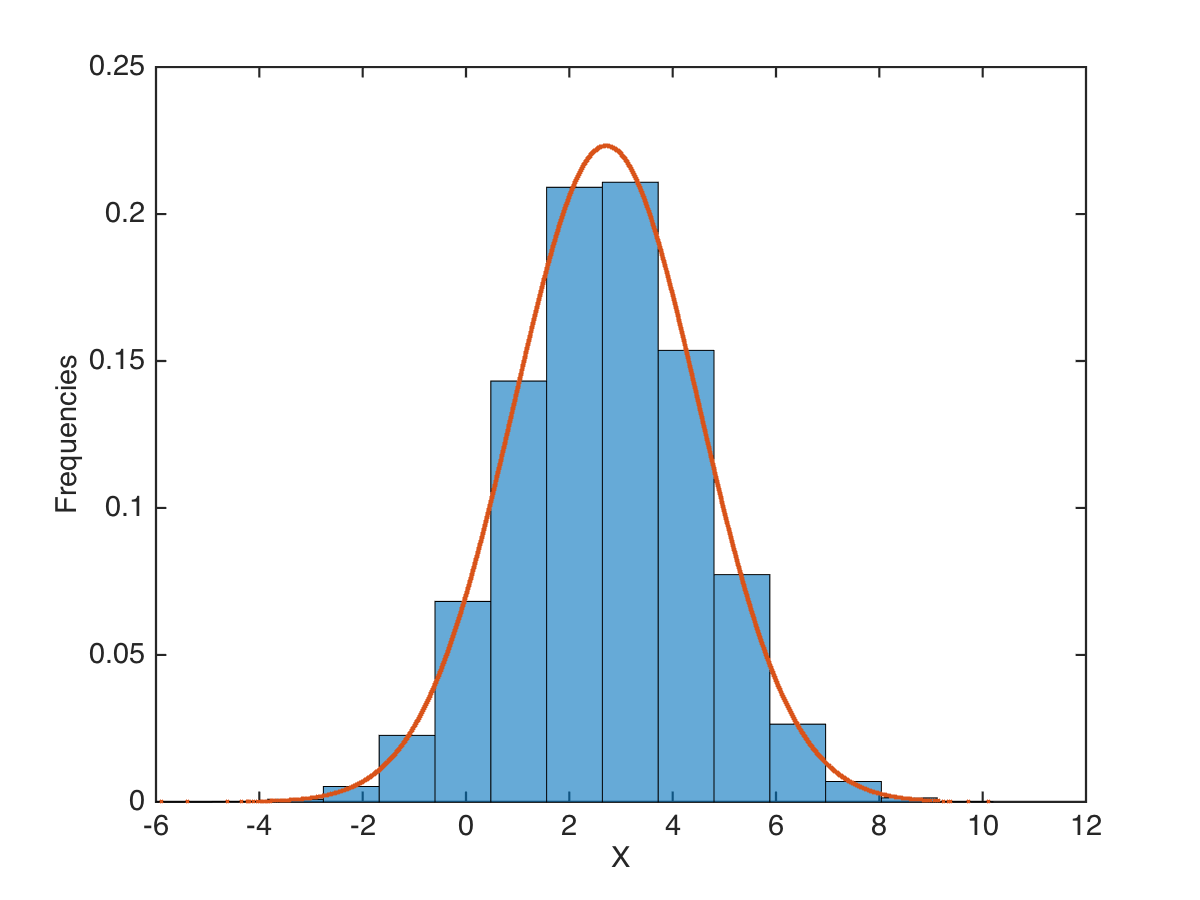
\includegraphics[width=0.5\textwidth]{Pictures/figure10.png}
\end{center}
\caption{Histogram of $X_t=1$.}
\label{fig3}
\end{figure}
\end{enumerate}


\section{Comparison of Random-Walk Metropolis and MALA}

The source code is in "main5$\_$sample$\_$comparisonMALAandRW". The simulation reproduces~\cite{sanz2014markov}[Figures 11 and 12].  This section should provide an introduction on the MALA algorithm and on the efficiency comparison of two methods.

We seek to sample the Boltzmann distribution with density ${\rm e}^{-V(x)}$ in $d$ dimensions with energy
\[
V(x) = \frac{k}{2}(r(x) - 2)^2, \quad r(x) = \| x\|_2, \quad k=100.
\]

The Metropolis adjusted Langevin algorithm (MALA) takes as a proposal the Euler-Maruyama discretization of (under this distribution) invariant the SDE
\[
dX_t =-\frac{1}{2}\nabla V (X_t)dt+ dB_t, 
\]
and corrects the sample by Metropolis-Hastings rule. More precisely,  the proposal is 
\[
\tilde{X}^{n+1} = X^n -  \frac{\Delta t}{2} \nabla V(X^n)  + \sqrt{\Delta t} Z^n,
\]
which is accepted with probability
\[
A_{\Delta t} = \min \left( \frac{\rho(\tilde{X}^{n+1}) T(\tilde{X}^{n+1}, X^n)}{{\rho({X}^{n}}) T(X^n, \tilde{X}^{n+1})} , 1 \right), 
\]
with
\[
T(X, \tilde{X}) = \left(\frac{1}{2\pi \Delta t}\right)^{d/2}{\rm exp}\left(- \frac{\| \tilde{X} - X + \frac{\Delta t}{2}\nabla V(X)  \|^2}{2\Delta t}\right)
\]


In order to compare the efficiency of the MALA algorithm with the random walk Metropolis-Hastings, we compare their empirical auto-covariance coefficients. The results in Figure~\ref{comparisonMALARW} suggest that Random walk Metropolis performs worse than MALA.
\begin{figure}
    \centering
    \begin{subfigure}[b]{0.45\textwidth}
        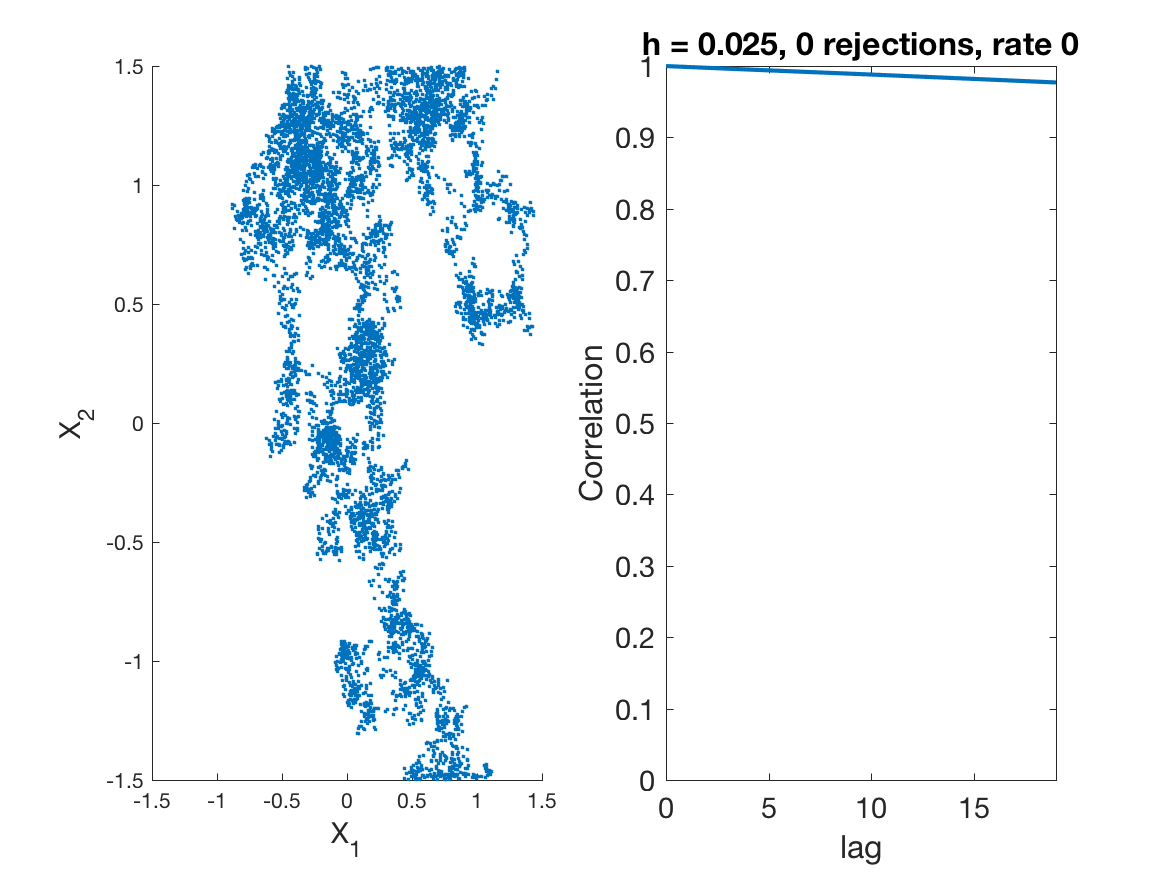
\includegraphics[width=\textwidth]{Pictures/figure11.png}
       \end{subfigure}
    ~    
     \begin{subfigure}[b]{0.45\textwidth}
        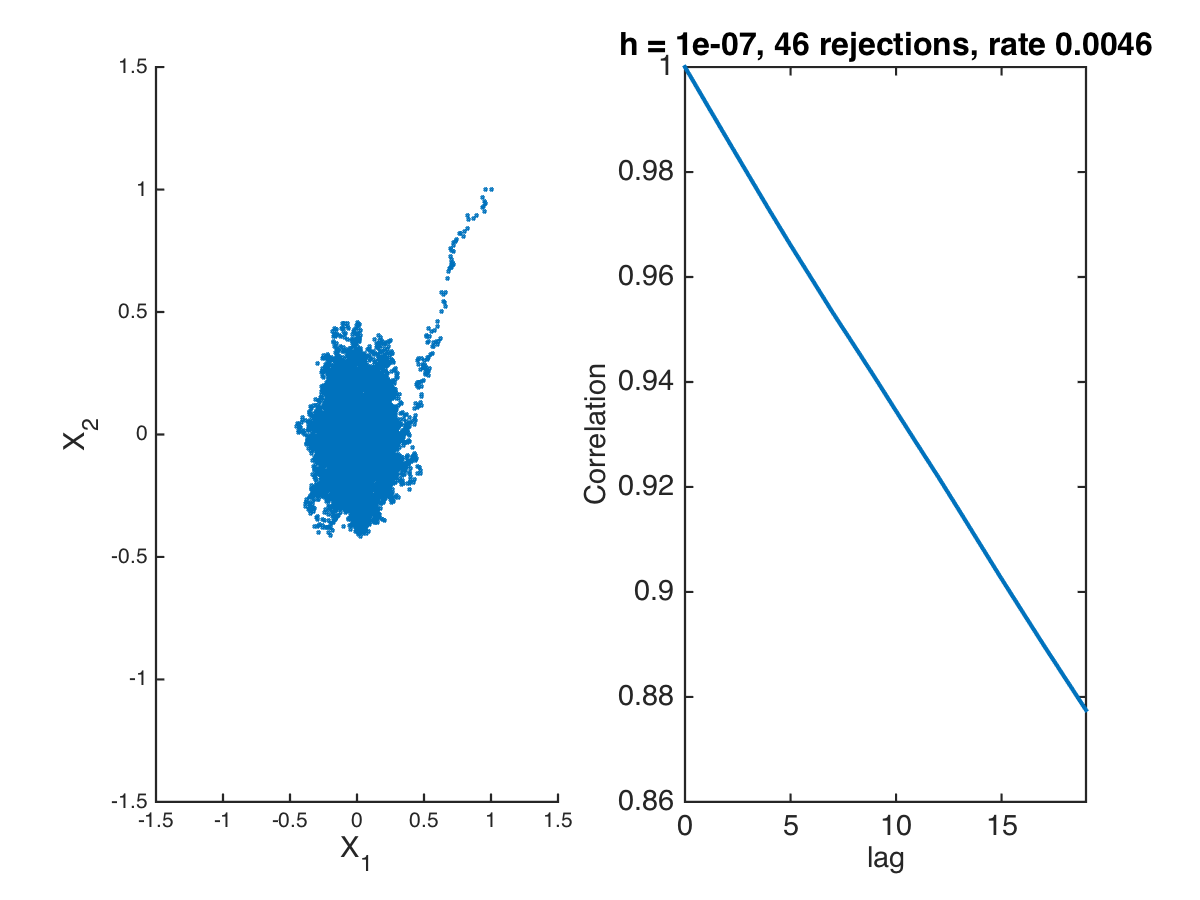
\includegraphics[width=\textwidth]{Pictures/figure12.png}
    \end{subfigure}
    \caption{Comparison of Metropolis Random Walk (Left) and MALA (right). MALA outperforms Metropolis RW.}
    \label{comparisonMALARW}
  \end{figure}
  Note that we have been tracking the average rejection, which is a very useful observable for Metropolized schemes and provides an information on the efficiency of generating successful proposals and can be tuned by changing the time step size. The bigger the time step, the bigger the rejection rate, i.e. the more proposals are refused and the correlations between the samples increase. On the other hand, a very small rejection rate might not be desirable neither, because it might require very small step sizes and therefore slow down the exploration again. Therefore, one should think about a good compromise, which will provide the best exploration. 
  
  \subsection{Tasks}
 
\begin{enumerate}
 \item Explain why can you see from Figure~\ref{comparisonMALARW} that MALA is better than Metropolis Random Walk.
\item Find the most efficient time step size for MALA (you might want to create a separate MATLAB main file, use "main5$\_$sample$\_$comparisonMALAandRW" as template) and name it main$\_$MALA$\_$findBestStepSize: 
\begin{itemize}
\item Write a "for-loop" iteration over time step sizes $h=0.01:0.01:0.2$ and simulate $10000$ steps of MALA.
\item Fix $20$ lag values between $0$ and $19$ and compute the empirical auto-covariance coefficient $\rho_{\nu}$ for every trajectory with step size $h$ and save the end values, i.e. $\rho_{\nu}$ at $\nu=19$.
\item Generate a plot of the average rejection rate and $\rho_{19}$ over the step sizes $h$. Which $h$ is optimal?
\end{itemize}

\end{enumerate}


\section{Comparison of Random-Walk Metropolis, MALA and HMC}

The source code is in "main6$\_$sample$\_$comparison$\_$RW$\_$MALA$\_$HMC". The simulation reproduces~\cite{sanz2014markov}[Figures 14, 15 and 16]. 

The Hybrid Monte Carlo algorithm (also called Hamiltonian Monte Carlo or in short HMC) is described in~~\cite{sanz2014markov}[Section 9]. 
\begin{verbatim}
function [X, rejections] = sample_HMC(N, dt, T, V, dV , X0)
% HMC
% parameters : int N, number of steps
%              double dt, time step size
%              potential V, function
%              dV gradient of the potential V, function
%              initial condition X0 of size (d,1)
% return : trajectory X, array (d,N)

rejections =0 ;
% determine dimension from the initial condition
d = length(X0);
% initialize array of samples
X = zeros(d, N);
X(:,1) = X0;
% initialize array of momenta
p = zeros(d, N);

% Hamiltonian defined for X, p \in R^d
H = @(q,p) V(q) + 0.5*p'*p;

U = rand(1, N);

% number of inner steps
L = floor(T/dt);
if (L ==0)
    L=1;
end

%sample N steps
for n = 1 : N - 1
    
    % resample momentum
    pRand = normrnd(0,1, size(X0));
    %save previous values of positions and momenta    
    xn = X(:,n);
    pn = pRand;
    % save previous state
    xnOld = xn;
    pnOld = pn;
    
    % perform L steps of deterministic dynamics
    for ni = 1: L
        % proposal
        [X_proposal, p_proposal] = sample_Verlet(2, dt, dV, xn, pn);
        xn = X_proposal(:,end);
        pn = p_proposal(:,end);
    end
    
    %compute acceptance probability
    acceptanceProba =  min(1, exp(-H(xn,pn) + H(xnOld,pnOld)));
    
    %Metropolis rule
    if ( acceptanceProba < U(n+1))
        % refuse
        X(:,n+1) = xnOld;
        % reverse momentum
        p(:,n+1) = -pnOld;
        rejections = rejections+1;
    else
        % accept
        X(:,n+1) = xn;
        p(:,n+1) = pn;
        
    end
end
end
\end{verbatim}


\subsection{Tasks}
\begin{enumerate}
\item Modify the code for HMC, so that the time-step $\Delta t$ can be random.
\item Prove that for $\pi(dx, dp) = {\rm e}^{-\beta V(x)}  {\rm e}^{-\beta \frac{1}{2}p^TM^{-1}p}dxdp $ with a potential energy $V$ such that 
\[
\int_{\Omega} {\rm e}^{-\beta V(x)}dx <\infty
\]
and a constant mass matrix $M$, 
it holds that
\[
\mathbb{E}_{\pi} [p^TM^{-1}p] = \beta^{-1}.
\]
\item In the code "main6$\_$sample$\_$comparison$\_$RW$\_$MALA$\_$HMC" use the by HMC generated momenta trajectory  $(p^n)_{n=1, \ldots, N}$ to compute the mean value of the kinetic energy, i.e.
 \[
 T_{\rm kin}^N = \frac{1}{dN}\sum_{n=0}^{N-1}{(p^n)^T(p^n)}, \quad p^n \in \mathbb{R}^d.
 \]
 To what value does $T_{\rm kin}^N$ converge as $N$ goes to infinity?
\end{enumerate}





\newpage

\section*{MATH11197: Research Skills in Computational Applied Mathematics. }

\paragraph{Individual report}


This assignment counts for 25\% of the total assessment for the 
module. The general aim of this project is to illustrate  that you have 
understood the material of the paper \cite{sanz2014markov} through 
completing the individual tasks described in the \texttt{MATLAB} 
documentation. You should typeset your work using  \LaTeX. Your 
report should not be more than $12$ pages long including references 
(11pt fonts).  Your report should also contain an introduction to the 
topic and should explain clearly the different steps you followed in 
order to complete the different tasks. A conclusions section 
summarising your findings and discussing some other possible studies you could perform should also be included. 



Your work will be assessed according to the following criteria:
\begin{itemize}
\item    \textbf{Exposition} (mathematical accuracy, clarity, literary presentation, degree of coverage of the topic) 40\%;
\item    \textbf{Literature} (understanding, relating different sources, finding new sources) 20\%;
\item    \textbf{Originality} (examples cited or constructed, new treatments and proofs of standard results, simple generalisations, original researches) 20\%;
\item    \textbf{Scope of topic} (conceptual and technical difficulty, relationship with previous studies, relevance of material included) 20\%.
\end{itemize}
Please refer to the grade descriptors for more information
\vspace{.8cm}


%\paragraph{First part:} You are asked to complete the tasks outlined in the matlab documentation.In particular, marks associated with each task are
%\begin{itemize}
%\item Task 2.b (1) $5\%$ (2) $5\%$
%\item Task 3.a (1) $5\%$ (2) $5\%$  (3) $10 \%$
%\item Task 5.a (1) $5\%$ (2) $5\%$
%\item Task 7.a (1) $5\%$
%\end{itemize}
%
%
%\paragraph{Second part:} \emph{Application to sampling in high dimensions}
%\newline
%Consider the problem of sampling from a high dimensional Gaussian with  covariance matrix $\Sigma$ given by 
%\[
%\Sigma =\text{diag} (\sigma^{2}_{1}, \cdots, \sigma^{2}_{100}), \quad  \sigma_{i}=(i/100)^{2}.
%\]
%\begin{enumerate}
%\item Write down the Hamiltonian equations of motion using a quadratic kinetic energy function. In particular your Hamiltonian should be of the form  
%\[
%H=\frac{p^{T}p}{2}+V(x),
%\]
%where $V(x)$ needs to be chosen in the appropriate way in order to ensure that one is sampling from the desired distribution.  \hfill [$5 \%$]
%\item Write down the discretization of the Hamiltonian equations using the leapfrog method \hfill [$5 \%$]
%\item By studying the corresponding one step map, deduce what is the maximum  $\Delta t$  that one is allowed to use when discretising the Hamiltonian equations. \hfill [$10\%$]
%\item Compare the performance between the Random Walk Metropolis and the Hamiltonian Monte Carlo (with deterministic and random choice of $\Delta t)$. Possible  diagnostic tests include \hfill [$35 \%$]
%\begin{enumerate}
%\item Plot the outputs for different co-ordinates for the RWM and HMC
%\item Studying the autocorrelation function for different co-ordinates and different methods
%\item Plotting the sample mean as a function of the different co-ordinates 
%\item Plotting the standard deviation as a function of the different co-ordinates
%\item Plotting the distribution of the MCMC method against the true distribution (you can do this component wise since every component is independent of each other)
%\end{enumerate}
%\end{enumerate}






\paragraph{Deadline} The assignment is to be handed in to MTO by Friday the 23rd of February at 12am. You will also 
need to submit your  \texttt{MATLAB} code online through learn. 

\newpage
\bibliographystyle{plain}

\bibliography{bibliography}

 







	
    
\end{document}
